\section{Generalizing ``Caps''}

The thesis moreover chooses to generalize caps. We have chosen the cap object for the further examination since the cap mesh models are readily available in the Shapenet library~\cite{chang2015shapenet}
and it was also possible to obtain the real-world cap data. Blenderproc~\cite{blenderproc} is used to generate the synthetic cap dataset similar to Suzanne dataset.
Caps are chosen such that each of them have distinct shapes, designs and colors. The cap models are chosen from the Shapenet library~\cite{chang2015shapenet} library
as it possess rich object information including textures, as one can see in Table~\ref{table:cap_dataset} in page~\pageref{table:cap_dataset}.\\

\begin{table}[htb]
    \centering
    \begin{tabular}{ccccc}
        \hline
        \multicolumn{5}{c}{Cap Dataset Preview}                                                                                                                                                                                                                                                                                                                \\
        \multicolumn{1}{c}{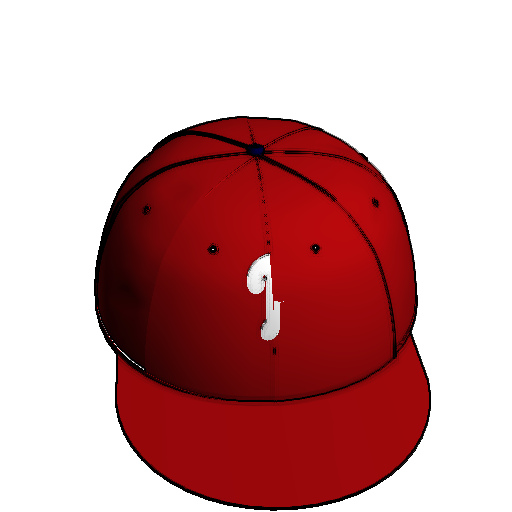
\includegraphics[scale=0.12]{images/cap/1.png}} & \multicolumn{1}{c}{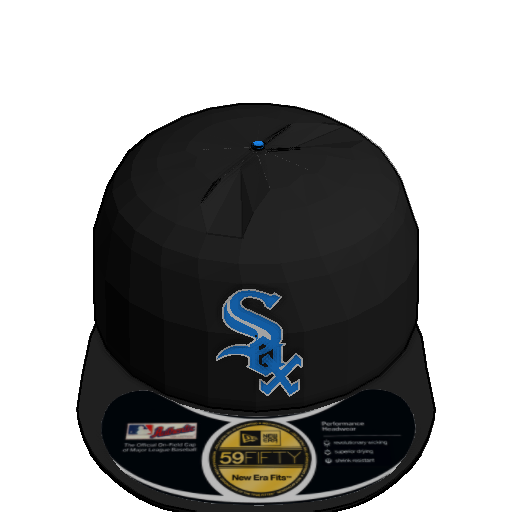
\includegraphics[scale=0.12]{images/cap/2.png}} & \multicolumn{1}{c}{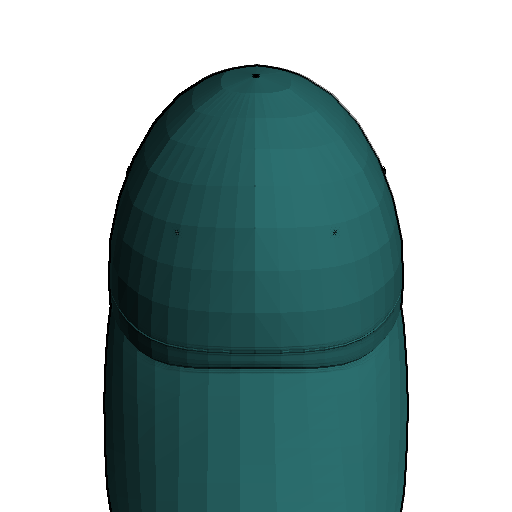
\includegraphics[scale=0.12]{images/cap/3.png}} & \multicolumn{1}{c}{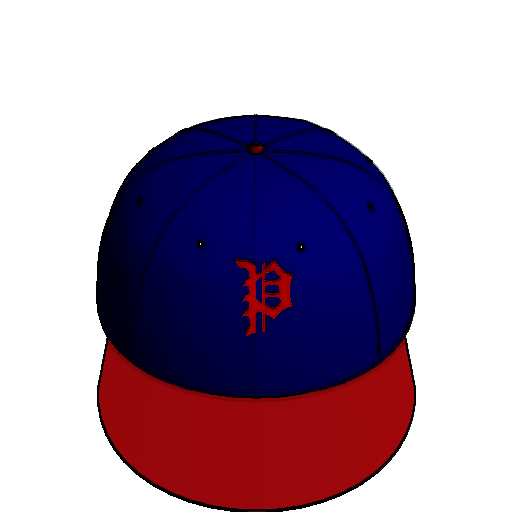
\includegraphics[scale=0.12]{images/cap/4.png}} & \multicolumn{1}{c}{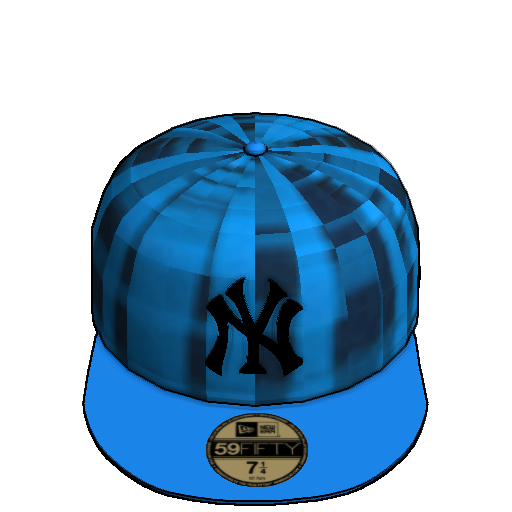
\includegraphics[scale=0.12]{images/cap/5.png}} \\ \hline
    \end{tabular}
    \caption{Illustration of caps sampled from the Shapenet library~\cite{chang2015shapenet}.}
    \label{table:cap_dataset}
\end{table}

To make the training more robust such that networks are more object-centric, the images are additionally augmented with random backgrounds and noisy backgrounds in
addition to color jitter and greyscaling augmentations, as depicted in Figure~\ref{fog:back_augmentations} in page~\pageref{fog:back_augmentations}. The mask information in the synthetic dataset is used to augment the backgrounds.

\begin{figure}[htb]
    \centering
    \caption{The image in the right illustrates the noisy backgrounds and the image in left describes random background augmentation.}
    \label{fog:back_augmentations}
    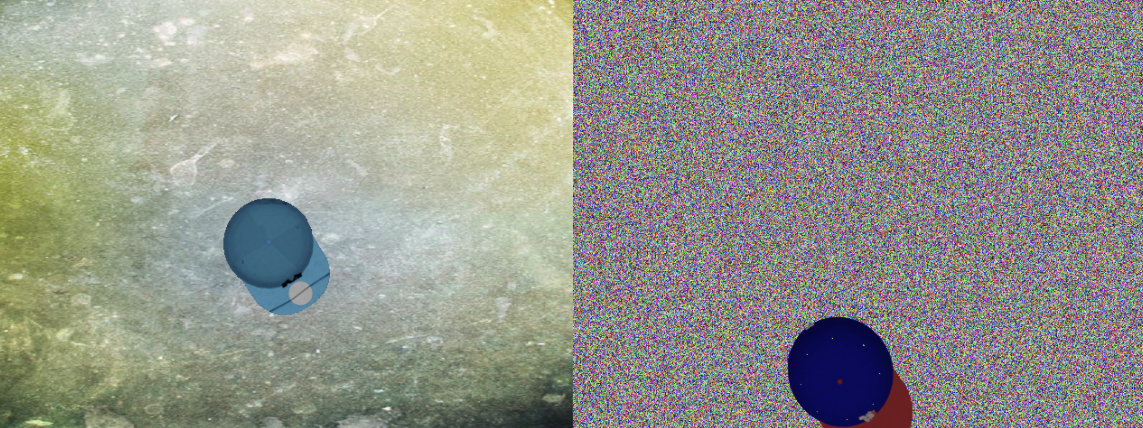
\includegraphics[scale=0.2]{images/cap/back_augs.png}
\end{figure}


\subsection{Semantic Correspondences Mapping Pipeline}

By definition, KeypointNet regresses semantic keypoints on the objects. Meaning, the keypoint in one object is positioned semantically equivalent in an another object of the same class.\\

Furthermore, this property of KeypointNet of producing semantic keypoints in the inference stage and not training phase can be used as correspondences in an image pairs to train \ac{DON}.
Loading semantic equivalent correspondences might affect the evalutaion of \ac{DON} based on $PCK@k$ metric.\\


\subsection{Tweaking the Training Pipeline}

Loading semantic correspondences to train \ac{DON} calls for a revision in the existing training pipeline. At first, the KeypointNet is trained to compute semantic correspondences
across objects belonging to the same class. The pretrained KeypointNet will be used to train \ac{DON}. Finally, we shall use the pretrained \ac{DON} to train the KeypointNet to sample geometrically
consistent single class generalized labels for robot grasping.
To the best of our knowledge, such a combination of the KeypointNet and DON is novel. \\

``End-to-End'' method of training the networks will not be used as the KeypointNet can only be trained using same object in an image pair
and not semantically equivalent object. Meanwhile, \ac{DON} can be trained using the semantic correspondences in an image pair.


\subsection{Evaluating Single Class Generalized Labels in the Wild}

The expression ``in the Wild'' denotes the case when the sampled single class generalized labels are evaluated against images which are not in the training pipeline.
The images of caps used for evaluation will be fetched from a smartphone camera.\\

Furhermore, the single class generalized labels for evaluation are autonomously picked from the KeypointNet trained on the \ac{DON} representation.\\


\subsection{Robot Grasping Pipeline}

To develop the robot grasping pipeline, Franka Emika 7-DOF robot manipulator is used. It is one of the robots available at sereact~\cite{sereact} equipped with hardware to run artificial intelligence algorithms.
The robot is equipped with the 2-jaw parallel gripper. Futhermore, Intel Realsense D435 camera is wrist-mounted as illustrated in Figure~\ref{fig:robot_setup}.\\

\begin{figure}[htb]
    \centering
    \caption{Robot setup for cap grasping with wrist-mounted camera.}
    \label{fig:robot_setup}
    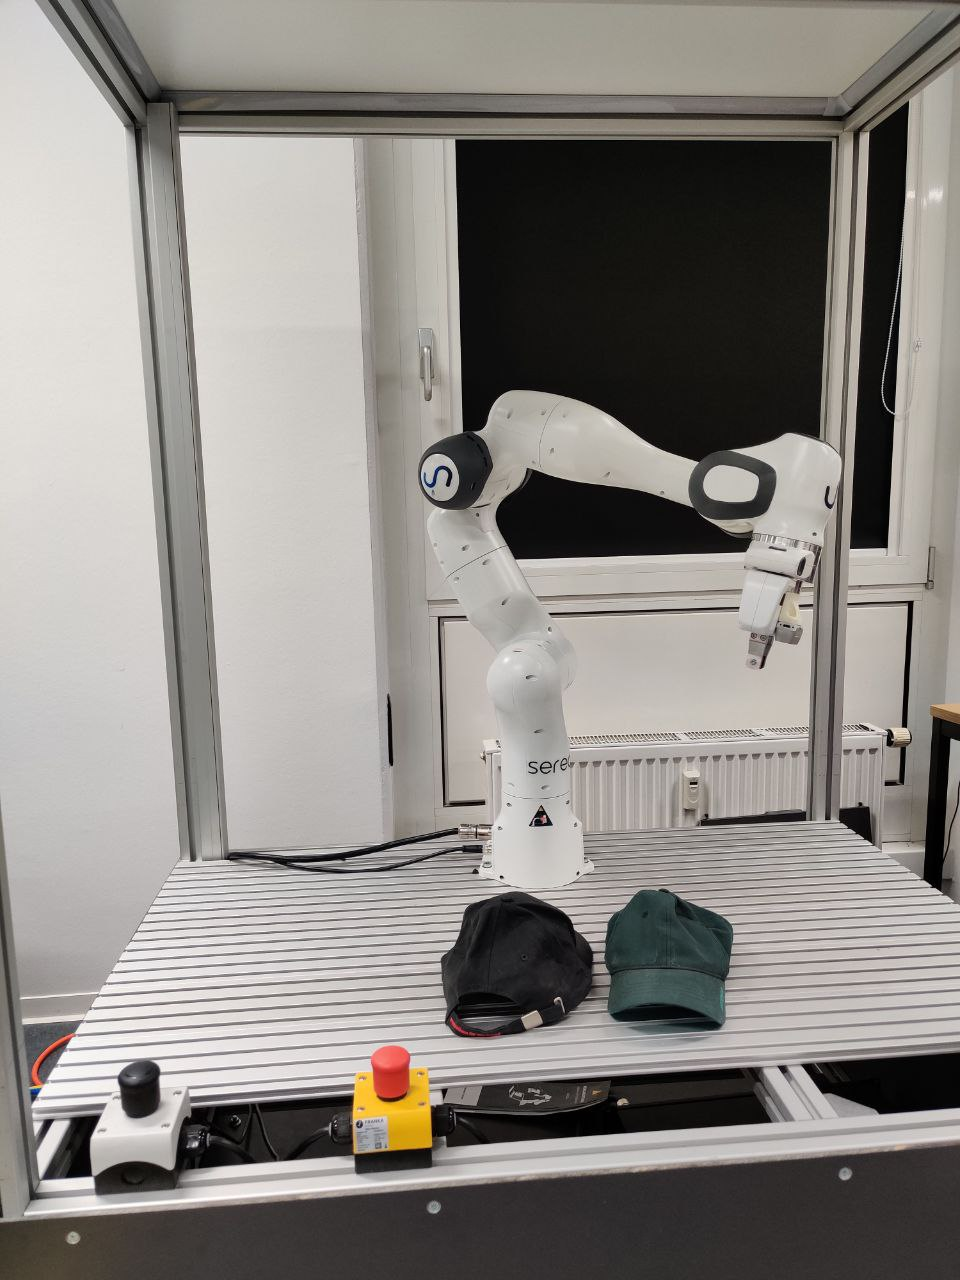
\includegraphics[scale=0.25]{images/robot/setup.jpg}
\end{figure}

The \ac{RGB} image is streamed into the neural networks to compute dense object descriptors from \ac{DON} and 6D pose produced from keypoints from the KeypointNet.
By using pre-computed single class generalized labels stored offline, the Guassian kernel from Equation~\ref{eqn:gaussian_kernel} in page~\pageref{eqn:gaussian_kernel}
is employed to produce grasping points for the robot. The depth information along with camera extrinsic and
intrinsic information is used to project the spatial expectation of the queried label (descriptor) to camera frame coordinate for robot grasping.